\chapter{System Design}
\section{Precision}
	It's important to have a clear definition of \de{\textit{precision}}, that's different from the concept of \textbf{\textit{accuracy}}: accurate can be seen as a synonymous of a \textit{correctness} (how close we are to the target we want to measure) when instead precise is a synonymous of \textit{consistent} (so when all measures are close together, but not necessarily near to the correct value). In general this two adjectives can be used together in order to create a \textbf{system} that's \textbf{accurate and precise}. In reality it's typically better to design a precise system instead of an accurate one: accuracy can be compensated/calibrated while instead a lack of precision cannot be overcome (and so the precision is an intrinsic property of the system itself).
	
	\begin{figure}[bht]
		\centering 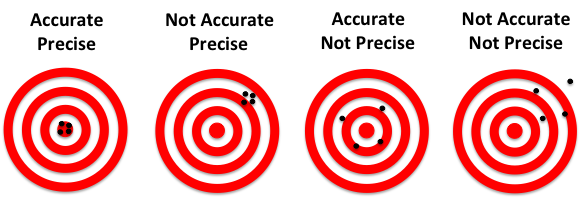
\includegraphics[width=8cm]{acc-prec}
		\caption{accuracy vs precision.}
	\end{figure}
	
	The design of a machine tool or a measurement system has to always consider the \textbf{11 principles for precision} that regards the following key concepts:
	\begin{enumerate}
		\item \textbf{structure}: the structure of the system needs to be stiff with high damping values in order to retain a certain rigidity and thus less degrees of freedom; aspect associated to the structure part are also related to the thermal stability of the system and it's seismic isolation;
		
		\item \textbf{kinematic/semi-kinematic design}: to create a more precisely reliable system  it's necessary to reduce redundant joint between different components (each part has 6 degrees of freedom, but using a joint with more constrains introduce some uncertainty that's the opposite of precision);
		
		\item \textbf{abbé principle}: when aligning measurement system it's important to follow this principle in order not to introduce unexpected side effects;
		
		\item \textbf{direct displacement transducers}: whenever possible it's preferable to measure with a direct transducer, not with a sensor that measure another property that's related to the property itself;
		
		\item \textbf{metrology frames}: this frames that are used to link together the component of the system should be involved in the measurements but should also avoiding the contact with external forces;
		
		\item \textbf{bearings};
		
		\item \textbf{drives/carriages}: in conjunction with the bearings, a system to be put in condition of measure needs to have component with high accuracy that limits the frictions and the thermal effects;
		
		\item \textbf{thermal effects}: whenever possible it's recommended to eliminate/minimise the thermal inputs and drift using stabilization or compensation methods;
		
		\item \textbf{servo drives and control} (CNC): this is a fundamental way to control motion in a repeatable and precise way, especially used in machining systems;
		
		\item \textbf{error budgeting}: in order to improve the way of the system works, it's important to classify different effects in order to understand the relative importance of each effect;
		
		\item \textbf{error compensation}: if it's possible to create a model of the error, it's always good to compensate for it.		
		
	\end{enumerate}
	
	In spite of this 11 principles we realize that, at a fundamental level, there will always be some noise that cannot be eliminated (but can still be reduced). This means that after having designed a system with improved precision it's important to \textbf{identify} and \textbf{quantify} the \textbf{causes leading to non-repeatability}: this is the statistical aspect of precision and represent the so called \textbf{industrial quality}.
	
	\subsection{Autocorrelation}
	
		This day almost all the measures are done using computer and electronic system, so if we consider a displacement sensor it's possible to measure a set of $n$ samples of displacement, each taken after a certain time $\Delta t$. Each sample $x_i$ will necessarily be different from the other, due to it's stochastic nature. At this point to estimate the \textit{real} length of the object to measure we can simply compute the average on the samples token:
		\begin{equation}
			\overline x = \frac 1 n \sum_{i=1} ^n x_i	
		\end{equation}
		This measure will be characterize with a certain variance $\sigma_x^2$; the mean value of the sample will also be a stochastic variable, and so by repeating the experiment itself we can retrieve the variance computed on $m$ measures of $n$ sample each:
		\begin{equation} 
			\sigma^2_{\overline x} = \frac{\sigma_x^2}{m}
		\end{equation}
		
		\begin{SCfigure}[1][bht]
			\centering 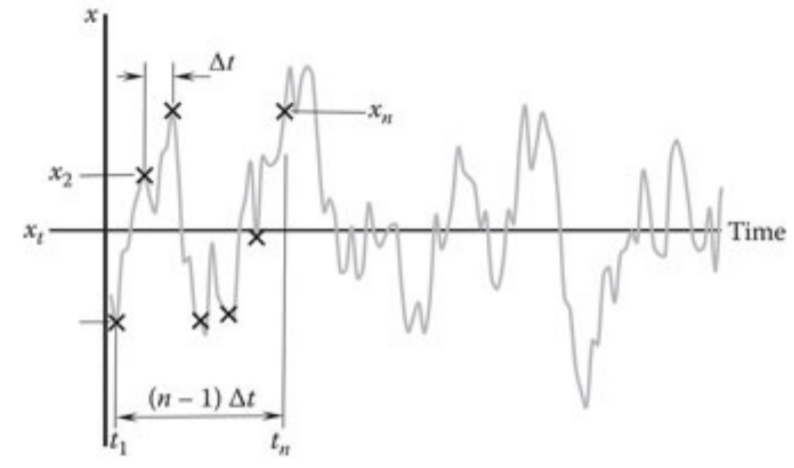
\includegraphics[width=5cm]{autocorrelation}
			\caption{example of values read by a displacement sensor in relation to the time $t$.} \label{fig:design:correlation}
		\end{SCfigure}
	
		As we might see in figure \ref{fig:design:correlation}, reading values in a little time span might result in a correlation between themselves (in fact if we consider a narrow sampling period $\Delta t$, the values registered by the system will be almost be equal), so by increasing the sampling time $\Delta t$ it's possible to get measures that are less correlated between each others. In particular, to solve this problem, it's possible to create the \de{autocorrelation function} $R_{xx}$ whose purpose is to define the minimum sampling time $\Delta t$ that generates uncorrelated data. This particular function is defined by computing the average of a signal with itself translated in time by a constant value $\tau$, so by doing
		\begin{equation}
			R_{xx}(\tau) = \frac 1{T-\tau} \int_0^{T-\tau} x(t) x(t-\tau) \, dt
		\end{equation}
		This particular function is interesting, because we can see that for $\tau = 0$ it simply compute the variance $\sigma_x^2$, however it happens that by incrementing the parameter $\tau > 0$ the function decrease following an exponential decay with time a time constant equal to $\tau_0$ and so the asymptotic value is zero; note that this behaviour is not a true value, but just an asymptotic limit, as it can be seen in figure \ref{fig:design:correlation-b}.
	
		\begin{SCfigure}[1][bht]
			\centering 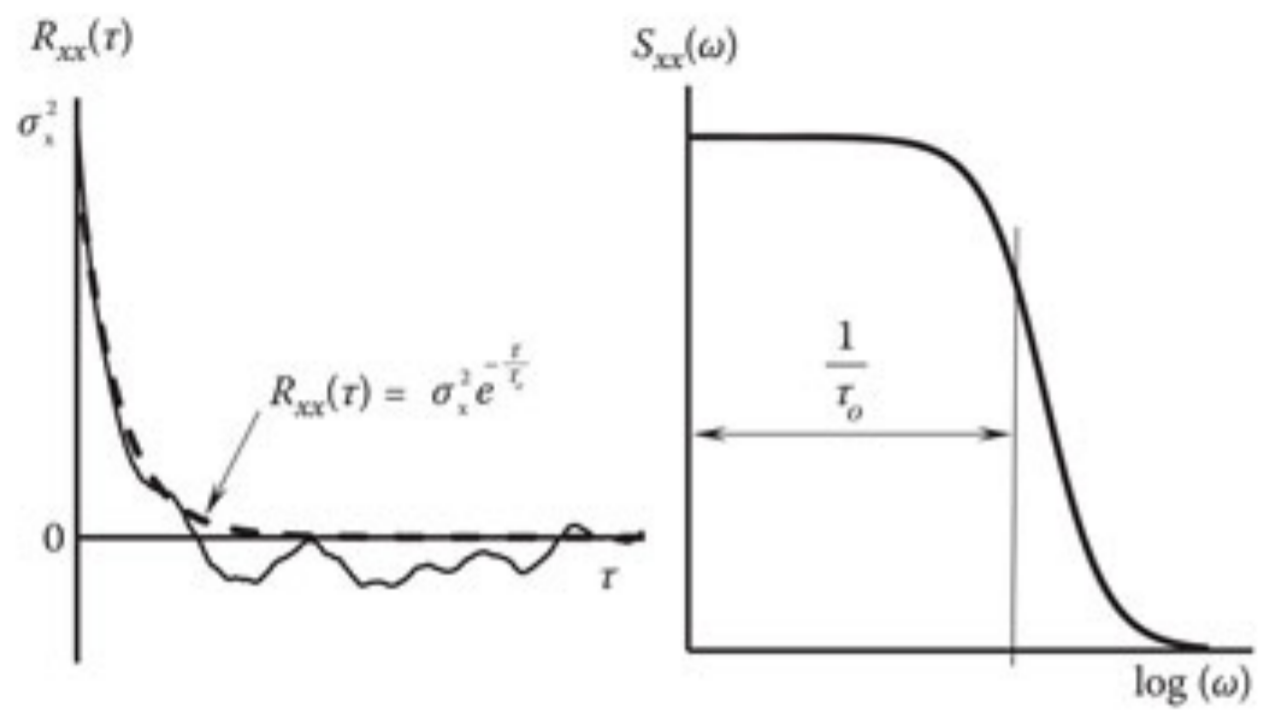
\includegraphics[width=5cm]{autocorrelation-b}
			\caption{trend of the function $R_{xx}$ and $S_{xx}$ read by an instrument.} \label{fig:design:correlation-b}
		\end{SCfigure}
		
		By considering the asymptotic value of the autocorrelation function, so by describing it as $R_{xx}(\tau) = \sigma_x^2 e^{-\frac{|\tau|}{\tau_0}}$ it's possible to compute the power spectral density $S_{xx}$ in the domain of the frequency that's equal to
		\begin{equation}
		\begin{split}
			S_{xx}(\omega) & = \frac{\sigma_x^2}{\pi} \int_0^\infty e^{-\frac{\tau}{\tau_0}} \cos(\omega \tau)\, d\tau = \frac{\sigma_x^2}{\pi \tau_0} \frac 1 {1 + (\omega \tau_0)^2} \\ & = \frac{S_0}{1 + (\omega \tau_0)^2}
		\end{split}
		\end{equation}
		This function is useful to determine that the value $\tau_0$ represents the \textbf{minimum sampling time} for consecutive samples to get the uncorrelated. Going back to the original statement of this section in order to get uncorrelated values we need to use a sampling time $\Delta t > \tau_0$.
		
		By this it consequent that, chosen a time $T$ on which the measure system saves data, the maximum number of uncorrelated sample that can be used for computing some specification on the system is equal to $n = T/\tau_0$, and so with them we can estimate the standard deviation $\sigma^2_{\overline x}$ on the averaged signal:
		\[ \sigma_{\overline x}^2 = \frac{\sigma_x^2}{T/\tau_0} \qquad \Rightarrow \quad \sigma_{\overline x} =\sigma_x \frac{\sqrt{\tau_0}}{\sqrt {T}} = \frac{P_0}{\sqrt {T}} = P_0 \sqrt{(BW)_m} \]
		As stated in this expression, by computing the square root on the variance it's possible to get the standard deviation of the system, and it's possible to see that's related to the \textbf{intrinsic signal noise} $P_0$ (property of the system) and to the square root of the acquisition time $T$ (if on denominator) or on the \textbf{measure bandwidth} $(BW)_m = 1/T$ (if on numerator). \\
		Note that the standard deviation is related to the square root of the acquisition time, so to increase the deviation $\sigma_{\overline x}$ (and so the precision) by a factor of 10, it will require 100 times more time, with a significantly increase of costs.
		
	\subsection{Limits of precision}
		
		As yet described, a limit of precision is the cost because it limit the acquisition time $T$ that could have reduced the standard variation $\sigma_{\overline x}$, but this is not the lonely effect.
		
		Virtually all precision measurements pass through electronics that are subjected to the so called \textbf{Johnson's noise} that's related to the random movement of the atoms that compose the structure, and so in general it depends on the temperature $T$ of the system. Consider for example a resistor $R$, it's thermal noise $P_{0,V}$ depends also on the Boltzamnn's constant $k = 1.38\cdot 10^{-3} J \cdot K^{-1}$ and the sampling bandwidth $(BW)_s$ as described by the equation
		\begin{equation}
			P_{0,V} = 2 \sqrt{RkT (BW)_s}
		\end{equation}
		
		When combining many electric and passive components, their noise sum up to combine into \textbf{pink noise} (like a white noise, but with more components on higher frequencies) whose spectral density is defined by the function
		\[ G(f) = \frac C f + G_0 \]
		Integrating this function over the frequency band of interest gives the variance $\sigma^2_V$ associated to this particular kind of noise
		\begin{equation}
			\sigma_V^2 = \int_{f_1}^ {f_2} G(f)\, df = C \ln \left( \frac{f_1}{f_2} \right) + G_0 \big(f_2-f_1\big)
		\end{equation}
		The truth that this equation wants to tell us it that is difficult to maintain precision over a long time, because the difference of frequencies $f_2-f_1$ (multiplied by $G_0$) will increase the variance.
		
		Another phenomenon that limit the precision of an instrument is the granular nature of current (that's made of flowing electrons); this effect is dominant for high currents $I$ and bandwidth $(BW)_s$ and determine a so called \textbf{shot noise} $P_{0,I}$ that's equal to		
		\[ P_{0,I} = \sqrt{2qI (BW)_s}\]
		where $q = 1.602\cdot 10^{-19} C$ is the charge of an electron.		
		\vspace{3mm}
		
		Pink noise and shot noise are the limiting factors on precision measurements where a phenomenon is converted through a transducer into a voltage or current. Much better precision can be exploited by converting a phenomenon into a value through time (needed, as example, for charging a capacitor or for a beam of light to travel a distance...) and not voltage/current; this time precision can reach value of $10^{-11} s$, increasing the precision of the overall system.
	
	
\section{System design}
	\de{System design} means giving a shape/architecture to a complex amount of components into a complex system that can be a full product (like a car) or just a subsystem of a bigger product (like an axil of a vehicle); in general dividing complex systems into subsystem is a trick to design products in a more manageable way. A good subsystem, to be so, should have the minimum connections/interfaces with the other components of the parent system. In system design we start from the needs of the problem and we architecture the system.
	
	Generally speaking, system design is strongly related to the \textbf{costs} of the project itself; in the design we can define three main phases:
	\begin{enumerate}
		\item determine and acknowledging the requires and the specification of the machine;
		\item designing the concept of the system;
		\item designing the final product.
	\end{enumerate}
	
	\begin{SCfigure}[1][bht]
		\centering
		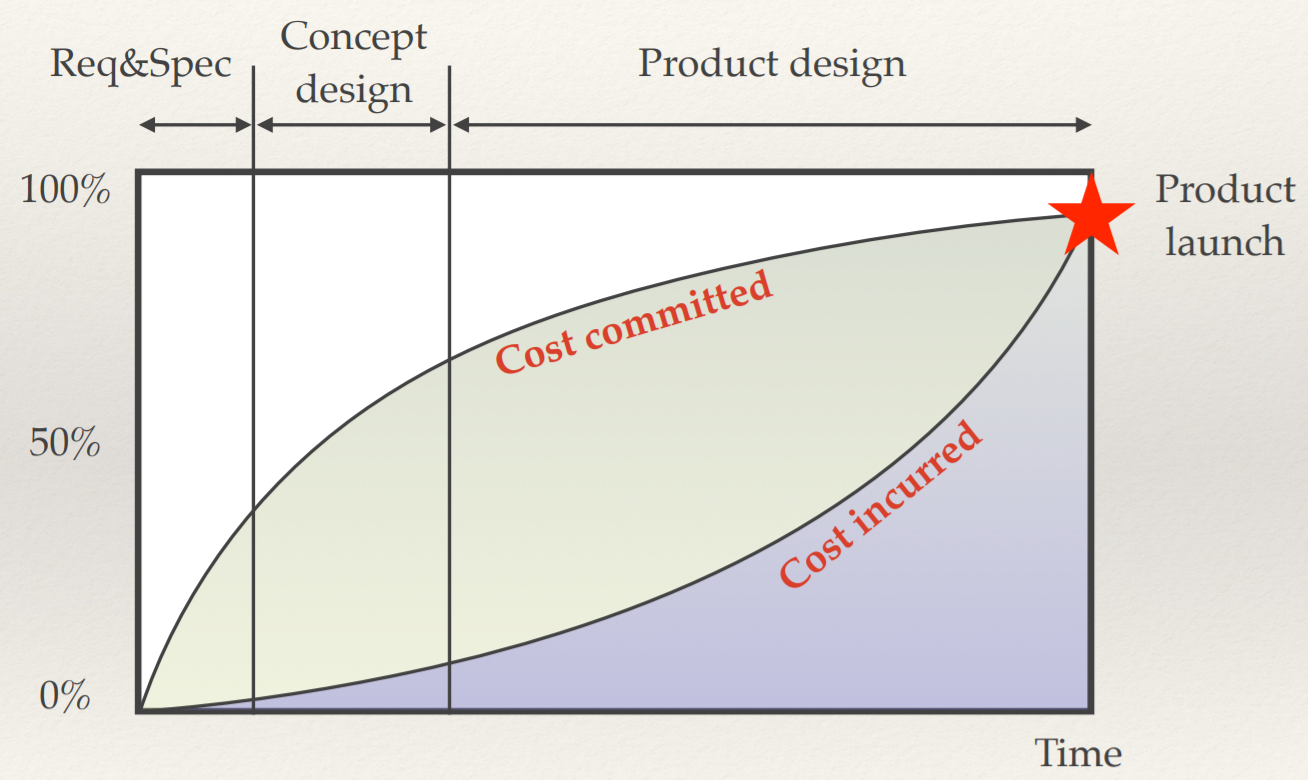
\includegraphics[width=6cm]{committed-incurred-costs}
		\caption{committed and incurred costs of a system design during the 3 phases.}
		\label{fig:des:commincurr}
	\end{SCfigure}
	
	As seen in figure \ref{fig:des:commincurr}, we can see that there are two principles \textbf{costs}: the \textbf{incurred} one, associated to the actually spent money on the project, and the \textbf{committed} one, associated to design decision made (like for example by determining the choice of a material, you will automatically create a future cost of production).
	
	The chart in figure \ref{fig:des:commincurr} is in conflict with the one in figure \ref{fig:des:knowfreed}: when you start creating your system, every possible choice is open and there is the maximum freedom; while developing the product it also increase the problem knowledge that, consequentially, limit the freedom. This is the so called \textbf{designer paradox}, and in general starting from zero knowledge can make the engineer take wrong decision: this will inevitably impact on the chart of costs by dragging them up. \\
	The best way is to have a problem knowledge curve that is as steeper as possible, while maintaining the freedom curve \textit{high} for the most time.
			
	\begin{SCfigure}[1][bht]
		\centering
		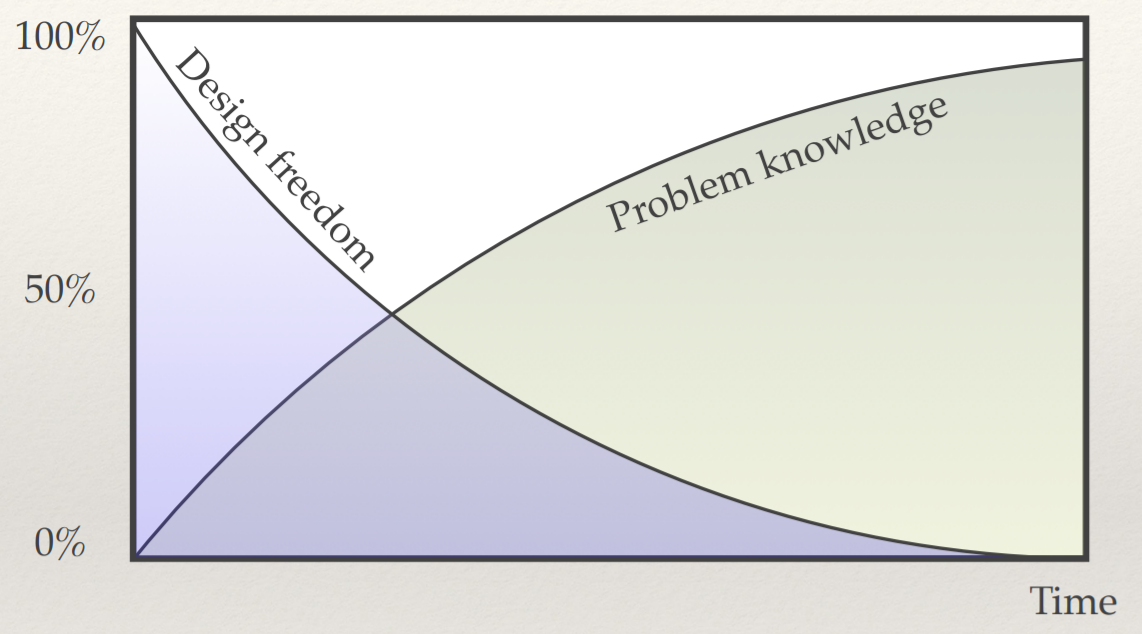
\includegraphics[width=6cm]{knowledge-freedom}
		\caption{design freedom and problem knowledge while designing a system.}
		\label{fig:des:knowfreed}
	\end{SCfigure}

	Another problem in system design is the human processing of the information, and in particular we can find the short term memory and the long term one. A good way to deal with huge problems is by decomposing them in order to store all the datas in long term memory a little by time.\\
	In a more practical way this states that initial design steps are critical and so it is fundamental to clearly state and understand the target of our design process, and also its constraints. The division of system into subsystems comes handy in this way, in order to subdivide more manageable tasks (that can be handled by the short term memory).
	
	\subsection{QFD: House of Quality}
		One of the best way to solve the first problem linked to the lack of problem knowledge is by using the so called \textbf{\textit{Quality Function Deployment Diagram}} \de{QFD}, also known as the \de{House of Quality} (name related to the shape of the diagram) shown in figure \ref{fig:des:qfd}.
	
		\begin{figure}[bht]
			\centering 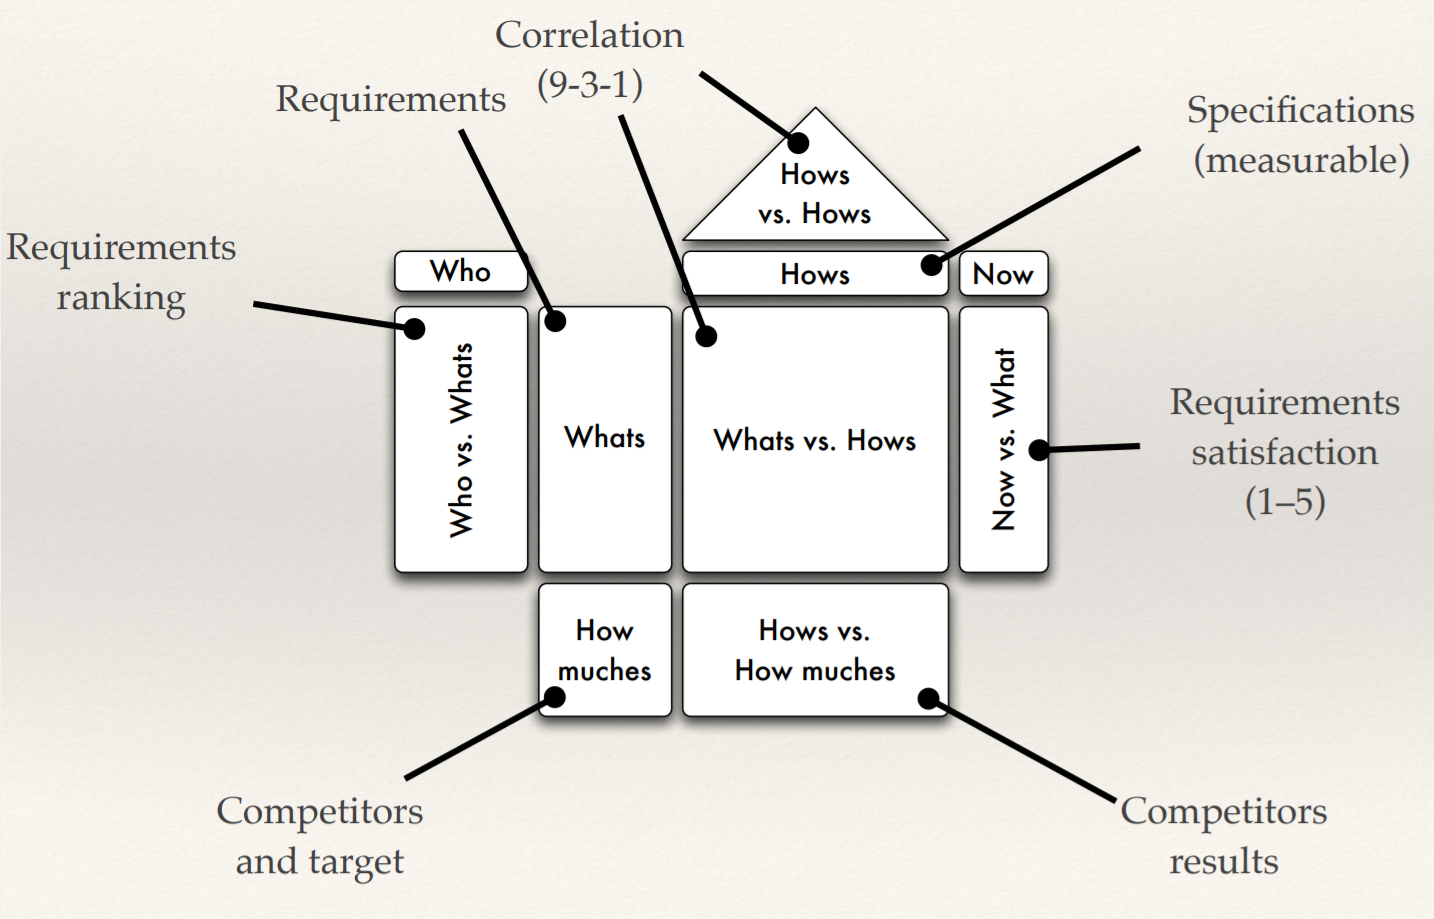
\includegraphics[width=8cm]{housequality}
			\caption{general diagram of a house of quality (QFD).}
			\label{fig:des:qfd}
		\end{figure}
		
		This diagram consists in table of multiple vectors containing different values and meanings; in particular we can find the following important vector containing the choices about:
		\begin{itemize}
			\item the \textbf{whats}: this are the \textit{customer requirements}, so a desired set in the product required by the customer;
			\item the \textbf{whos}: this are the customer of the product that can be the buyers, but also the sellers, the maintenance personal... (in general all the people that are reached by the product);
			\item the \textbf{hows}: this are the engineering specification of the system (related to the thing mentioned above). In particular we define the \textit{whats} as qualitative requirements, while the \textit{hows} are quantities;
			\item the \textbf{nows}: this are the competitors, so how the problem is already solved by other companies;
			\item the \textbf{how muches}: this are the target for our specification.
		\end{itemize}
		In general the (\textbf{customer}) \de{requirements} are the properties of product attributes stated by the customer and they always shall be: discriminatory (no space for doubt to know if the concept is good or not), measurable, orthogonal, universal and must be external (they should not depend on how the interior of the product works, like for example a car must be responsive in changing speed, not it's sizes and number of cylinders).
		
		On the other hand the \de{specifications} are quantitative and measurable criteria that the product is designed to satisfy; in general the specifications are internal attributes, like for example that a car has to accelerate from $0 km/h$ to $100km/h$ in less then $6s$.
		
		\paragraph{Who} The first thing to do to create a QFD is by expliciting the customers that can be both external (to the organization, like the consumer) or internal. In general it's useful to find the main customer of the product.
		
		\paragraph{What} The second step is to identify the customer requirements and this can be very tricky. In this step it's useful to see the \textbf{Kano's diagram} (figure \ref{fig:des:kano}) that shows the customer satisfaction in respect to the product function. In particular by time passing, the customer satisfaction passes from the green light to the red one, and this depends on the particular technology. By this sense, it's important to implement something that satisfies the customer more.

		\begin{SCfigure}[0.6][b]
			\centering
			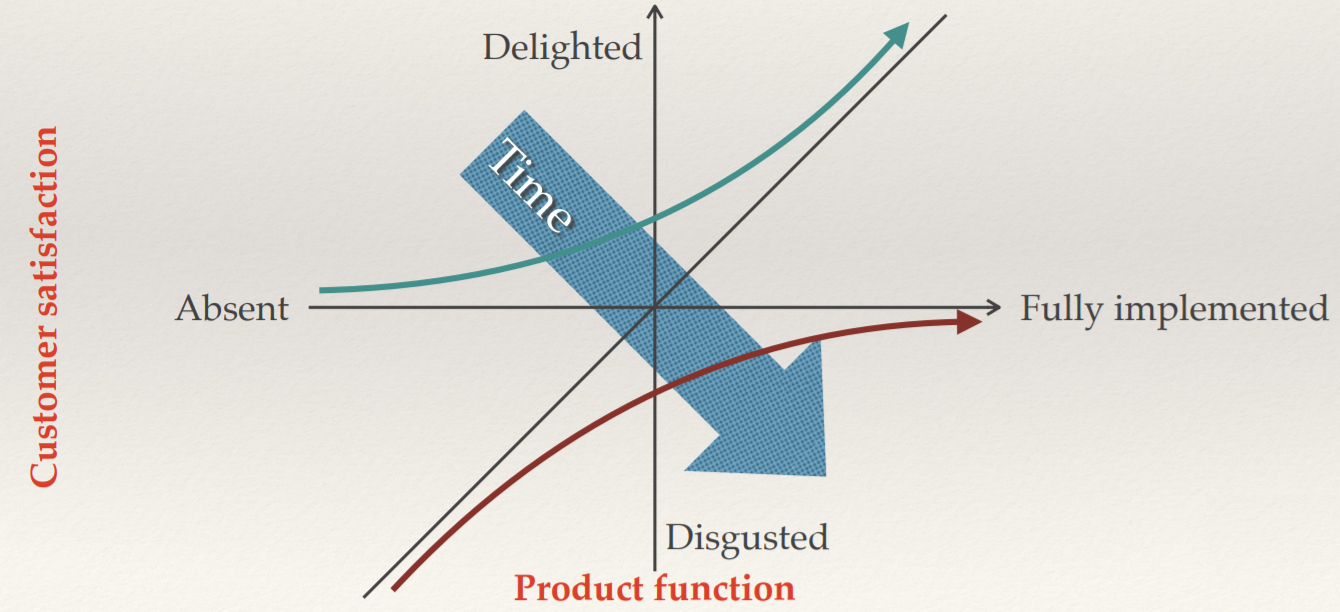
\includegraphics[width=7cm]{kano}
			\caption{Kano's diagram.}
			\label{fig:des:kano}
		\end{SCfigure}
		
		At this stage it's possible to see 5 different types of requirements:
		\begin{itemize}
			\item the attractive requirements, made to turn on delightment;
			\item one-dimensional requirements associated to performance of the product;
			\item mandatory requirements (red line in diagram \ref{fig:des:kano}) that are necessary to avoid the risk of disgustment;
			\item indifferent requirements that are not necessary to the main customer, but are worth for secondary customer;
			\item the reverse requirements that are valid for other customer in contradiction (like someone wants a handle light, someone heavy). In general a design is always a trade-off of requirements contradictions.
		\end{itemize}
		In general the way to identify the customers requirements are by using collection methods (surveys of random people or by using focused groups), or by collecting them in general therm (no jargon) that are then translated in engineering form. \\
		The customer requirements can be: functional, related to human factors, physical, time-related (in a general way \textit{reliability}), lifecycle related, resource.
		
		\paragraph{Who vs what} The third step is to create a matrix comparing the whos and the whats of the product; this can be done by determining a relative importance of the various aspects by weighting and ranking the attributes. Traditionally we create an absolute ranking (1 to 10) of the requirements, but to avoid to give high rank to a lot of requirements, than a good idea is to allocate a fixed sum (100 points for example) to the attributes.
		
		\paragraph{Now} At this time we create a list of raw competitors and do a benchmarking (to create the now vs what column). This stage asses how every competitor comply with the requirements by rating existing design, for example, from 1 to 5.
		
		\paragraph{How} The fifth stage is to generate the engineering specifications, so how a certain requirement will be met. For every requirement it's necessary to generate as many as possible engineering parameters suitable for measuring it. If it's not possible to find a proper measurement unit, than this is not a specification of the design. For each specification it's necessary to add a direction of improvement.
		
		\paragraph{How vs what} At this time we can create a matrix relating the hows to the whats, and in particular defining the degree of relationship between the two data (for example a blank cell might describe no relation between the attributes, $\square$ might indicate a weak relation, $\ocircle$ a medium weigth relation and $\odot$ a stronger one).
		
		\paragraph{How much} On the bottom of the QFD we set the engineering target, measured if possible as a range (a minimum value that's related to \textit{disgusting} and a max value associated to \textit{delighted}), and if possible by confronting this results with the competitors.
		
		\paragraph{How vs how} This is a cross correlation matrix (that's why it's triangular) that's used to identify relationship between specifications by identifying duplicates and the trade-offs. This triangular matrix should be filled with values/symbols representing the degree of relationship.
		
	\subsection{Concepts generation}
		Now that we have created and populated the house of quality we need to gradually move from the problem description to the product design that satisfies all the requirements. This process should be gradual because it's usually an error to going straight to a final solution: by doing so we might fall in love with the first idea without realizing its shortcomings. We rather wont to move from the QFD to a high number of \de{concepts} to product design.
		
		In general a concept is a rough, sketchy description of physical principles which an idea is based on, but detailed enough to understand the physical principles that determine the system itself. The concepts can be generated by:
		\begin{itemize}
			\item a \textbf{functional decomposition} where the overall task is split into atomic functions;
			\item a \textbf{morphology combination}: for each atomic function it's necessary to find out two or more possible implementation of the same function, then combine different implementations into a multitude of concepts. In general this step can be iterative, in a sense that if a function is not atomic, this can be subdivided another time. By following this approach it's possible to have a very high number of concepts, but in this case it's important to keep in mind the only one that really make sense (not all the combinations are good).
		\end{itemize}
		
		Functional decomposition can be helped by the \textbf{product decomposition} if there's already an example product (to train you take an existing product and you virtually disassembly it); to find this implementation we can use literature/market/patent searches, analogies, extremes and inverses (of a property/attribute, like changing order/position/dimension of a component) and by using the TRIZ method (that will be described in the next paragraph).\\
		Product decomposition is useful while re-designing an already exsisting system: this process can be done by removing one component at a time and, by doing so, documenting the associated loss of function. Later it's possible to create a table reporting, for each component, its connections and associated loss of function. By determining the function lossed, by reversing the idea we can get the atomic function that determine the original product.
		
		\paragraph{TRIZ} A method to create concept variance is the TRIZ method (translated from russian as \textit{Theory of The Resolution of Invention-Related Tasks}) developed by Genrikh Altshuller: by following this method it's possible to go straight from the problem to the solution. This is done by analysing pattern in patents for solution by sorting them by function rather then application.	\\
		The aim of the system is to avoid the need for inspiration and trial \& error procedures and systematically find new ideas. At the core of this system there are contradictions and inventive principles. In the design there are always contradictions that can be solved as trade-offs (like the weight/stiffness one); to help this problematic it's possible to use a $39\times 39$ matrix (that can be found at \url{http://www.triz40.com/}) of features/parameters that can combines into contradictions: each cell reports one (or more) of the 40 inventive principles that can be used.
		
	\subsection{Concept selection}
		If all goes fine, at this point we have a handful of products concept available ($7\pm 2$) that are detailed enough to understand the physical laws and how the system should work. The problem at this stage is that we don't have enough knowledge, and so we need to create a method that is robust enough to compensate this lack; at first we shall analyse each concept individually and reject it if it's clearly defective, and only later compare them. At this point is also necessary to consider the \textbf{safety} of the concept in terms of: intrinsic safety, presence of safety devices/countermeasures or precautions against improper use; this operation might give some feedback to functional decomposition preciously done.\\
		In this regard there is the military standard \texttt{MIL-STD 882B} that present a useful table that relates damage impact vs it's frequency.
		
		\begin{table}[bht]
		\centering
		\begin{tabular}{c c || c | c | c | c}
			& & \textbf{I} & \textbf{II} & \textbf{III} & \textbf{IV} \\
			& \textbf{Frequency} & Catastrophic & Critical & Marginal  & Negligible \\ \hline \hline
			A & Frequent ($>10\%$) & 1 & 3 & 7 & 13 \\
			B & Probable ($1-10\%$) & 2 & 5 & 9 & 16 \\
			C & Occasional ($0.1-1\%$) & 4 & 6 & 11 & 18 \\
			D & Remote ($0.001-0.1\%$) & 8 & 10 & 14 & 19 \\
			E & Improbable ($<0.001\%$) & 12 & 15 & 17 & 20 \\
		\end{tabular}
		\caption{\texttt{MIL-STD 882B} table.} \label{fig:des:milstd}
		\end{table}
				
		Each cell as a \textbf{risk} value ranging from 1 (high risk) to 20 (very low risk), where the acceptable values are $18$ or greater; values less then 5 are unacceptable while value ranging from 10 to 17 can be accepted with review.
		
		\vspace{3mm}
		
		After evaluating all the concepts by safety point of view and their feasibility (physical principles on the product have to be demonstrated and are technologically mature based on the \textbf{TRL} \textit{Technology Readiness Level} that has to be at least evaluated 7 to 9). Later it's possible to rank the concepts that is often made by using the \de{decision matrix}.
		
		The decision matrix is made by selecting some criteria  (from the QFD) and assigning them a weight that are going to be used to compare the concepts. At this stage it's important to pick a \textit{datum}, a reference that's used to create comparison. At this point, for each criteria and concept, it's possible to give scores ($1,0,-1$) and at the end calculating the result. In designing group every member should create it's tables interdependently in order to confront them at the end.\\
		The problem of this decision matrix is that the evaluation is made by people that could have a limited knowledge (in respect to some criteria); to avoid this problem it's more preferable to use the \textbf{robust decision making} that states \textit{"good decision are based on uncertain knowledge"}. In order to this method to work we need to use the \textbf{belief map} that take in account both the knowledge and the confidence of the judge. Mathematically we can describe the belief as a convex (?) function dependent on the knowledge level $p(k)$ and confidence $p(c)$:
		\[ \textrm{belief} = p(k)p(c) + \big(1-p(k)\big)\big(1-p(c)\big) \]		
		\begin{SCfigure}[0.6][b]
			\centering
			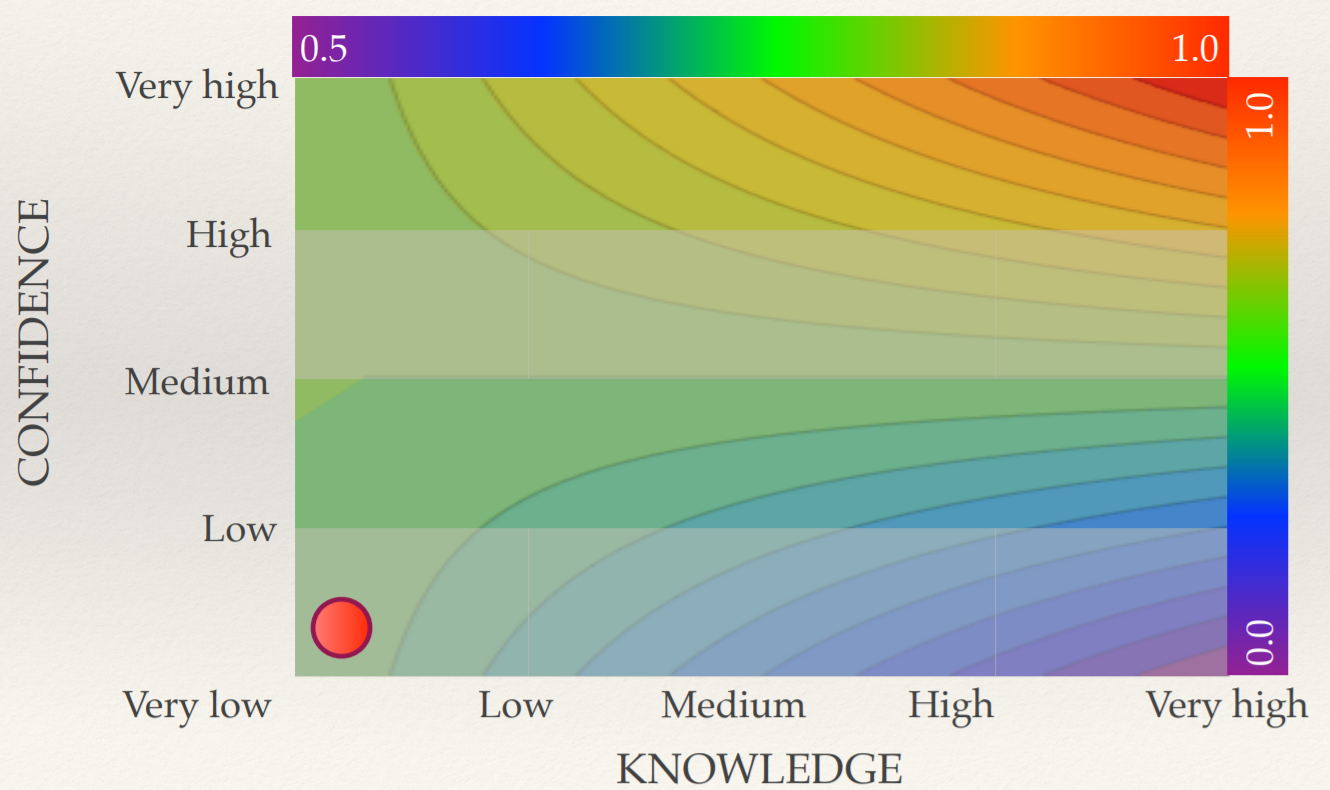
\includegraphics[width=7cm]{beliefmap}
			\caption{heat graph of a belief map.}
			\label{fig:des:beliefmap}
		\end{SCfigure}
		
		Now it's possible to use the belief value to fill up the decision matrix (and so not using the $\pm 1$ scores). At the end, for each concept, it's possible to compute the satisfaction level as
		\[\textrm{satisfaction} = \sum_i \textrm{belief}_i \, W_i \]
		where $W_i$ are the weight associated to the criteria.
		
		
		
		
		
		
		
		
		
		
		
		
		
		
		
		
		
		
		
		
		
		
		
		
		
		
	
